
\subsection{Data description}


\subsection{Estimation methodology}

\subsection{Abnormal returns in the market adjusted model}


\subsection{Short term abnormal returns in the Market Model}

To test hypothesis #1 and #2 of whether negative and positive SDG related events impacts firm value on the short term, we set apart negative and positive events and assess the aggregated development in abnormal returns 10 days before and 10 days after an event. Moreover, we isolate the effect of the individual SDGs to test hypothesis #4 of whether events on some sustainability goals are more relevant for investors than other. We apply the Market Model to measure abnormal returns around an event.   

\subsubsection{Positive news}

 
The average abnormal returns and cumulative average abnormal returns retrieved from the Market Model are illustrated in table \ref{ST_tab}. The development in AAR and CAAR, along with its corresponding standard error bands with a confidence interval of 95\%, is portrayed in figure \ref{fig:ST_pos_news} to support the analysis from a visual perspective. The y-axis depicts the abnormal return and the x-axis before and after an event. The effect of positive events on average stock behavior is presented by the blue line in the graph, and is mostly positive leading up to an event, which indicates a leakage effect. The positive AAR is especially pronounced between $t =-8$ and $t=-4$ before an event, and with a spike on the event date. However, when adjusting for the expected errors with assistance from the error bands, the AAR is only significantly positive and different from zero on $t= 0$ with an average abnormal return of 0.07\%. 

\begin{figure} [H] 
    \centering
    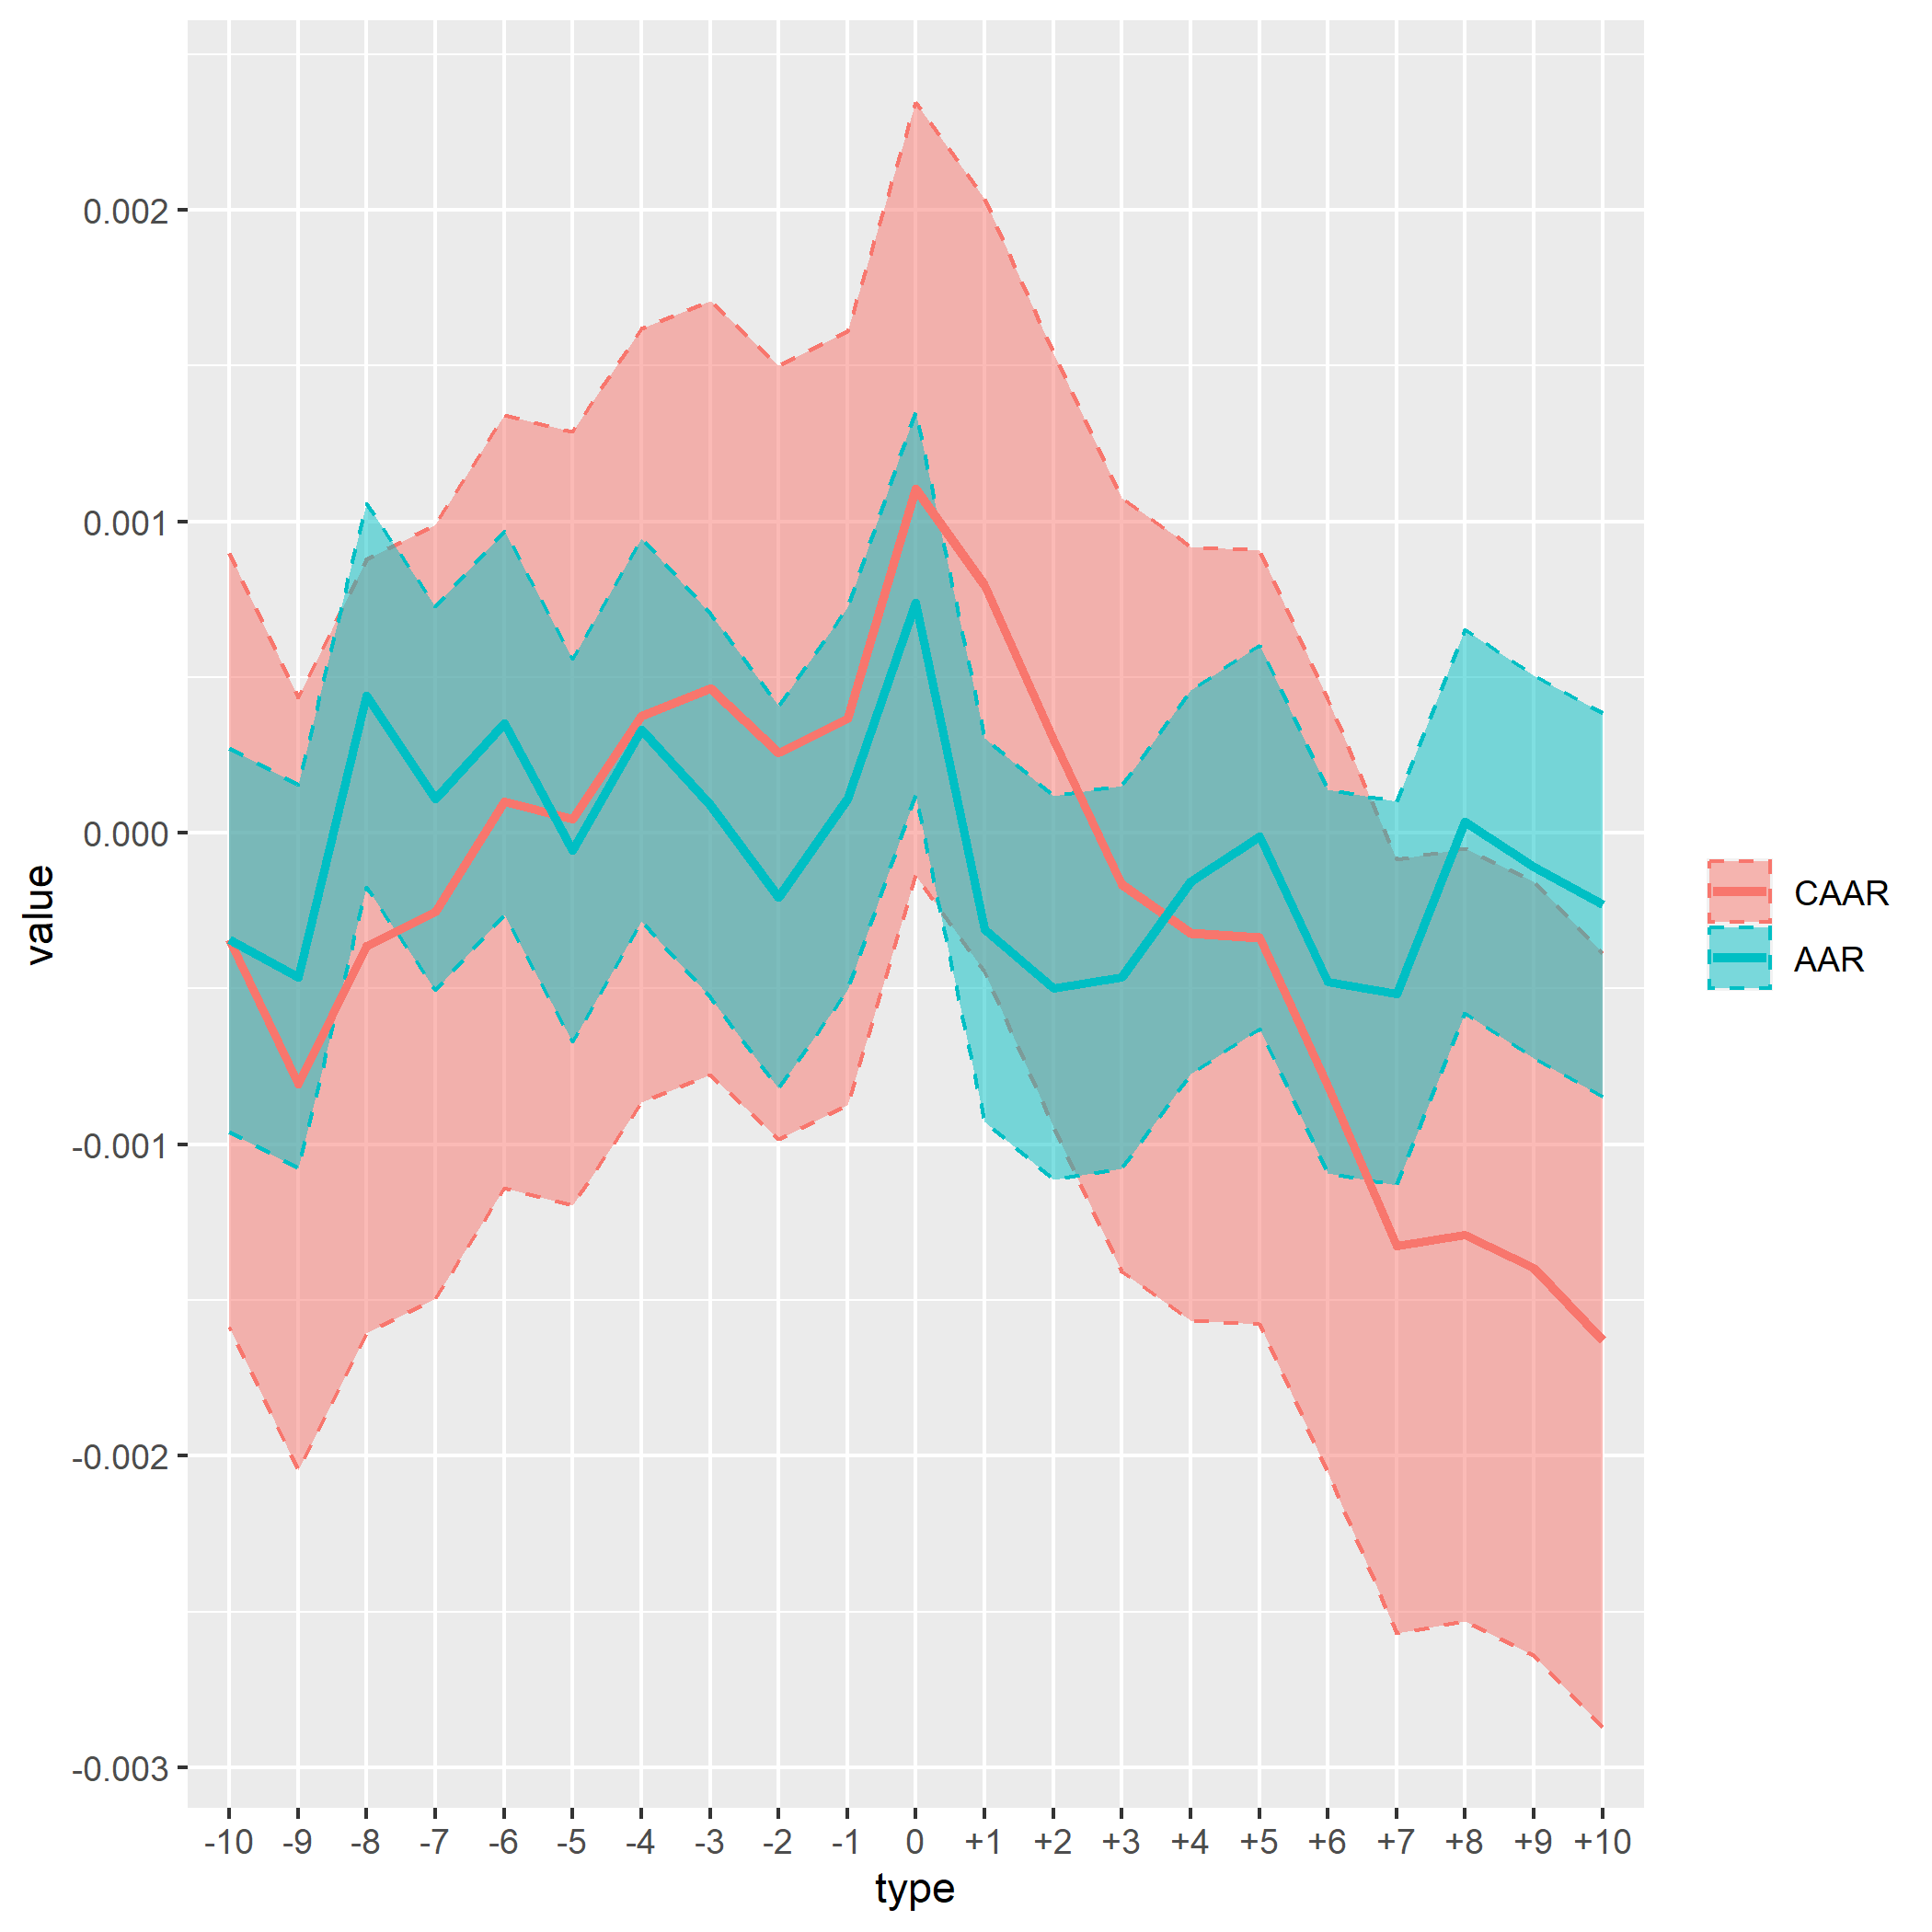
\includegraphics[scale=0.6]{Projekt/1.Figures analysis/ST_positive_all_CI.png}
    \caption{Short term positive news: AAR and CAAR}
    \label{fig:ST_pos_news}
\end{figure}

The positive AAR provides basis for a significantly positive and increasing trend in the CAAR (red line) leading up to and including the event date. However, at $t = 1$ and all subsequent days the AARs are slightly negative leading to a downward-sloping trend in CAAR, which eventually ends in significantly negative territory on $t = 10$ at $-0.16\%$.

 Examining the average effect from, respectively, positive and negative events provides insights into the overall tendency in shareholder sentiment on social responsibility. 

\begin{figure} [H]
    \centering
    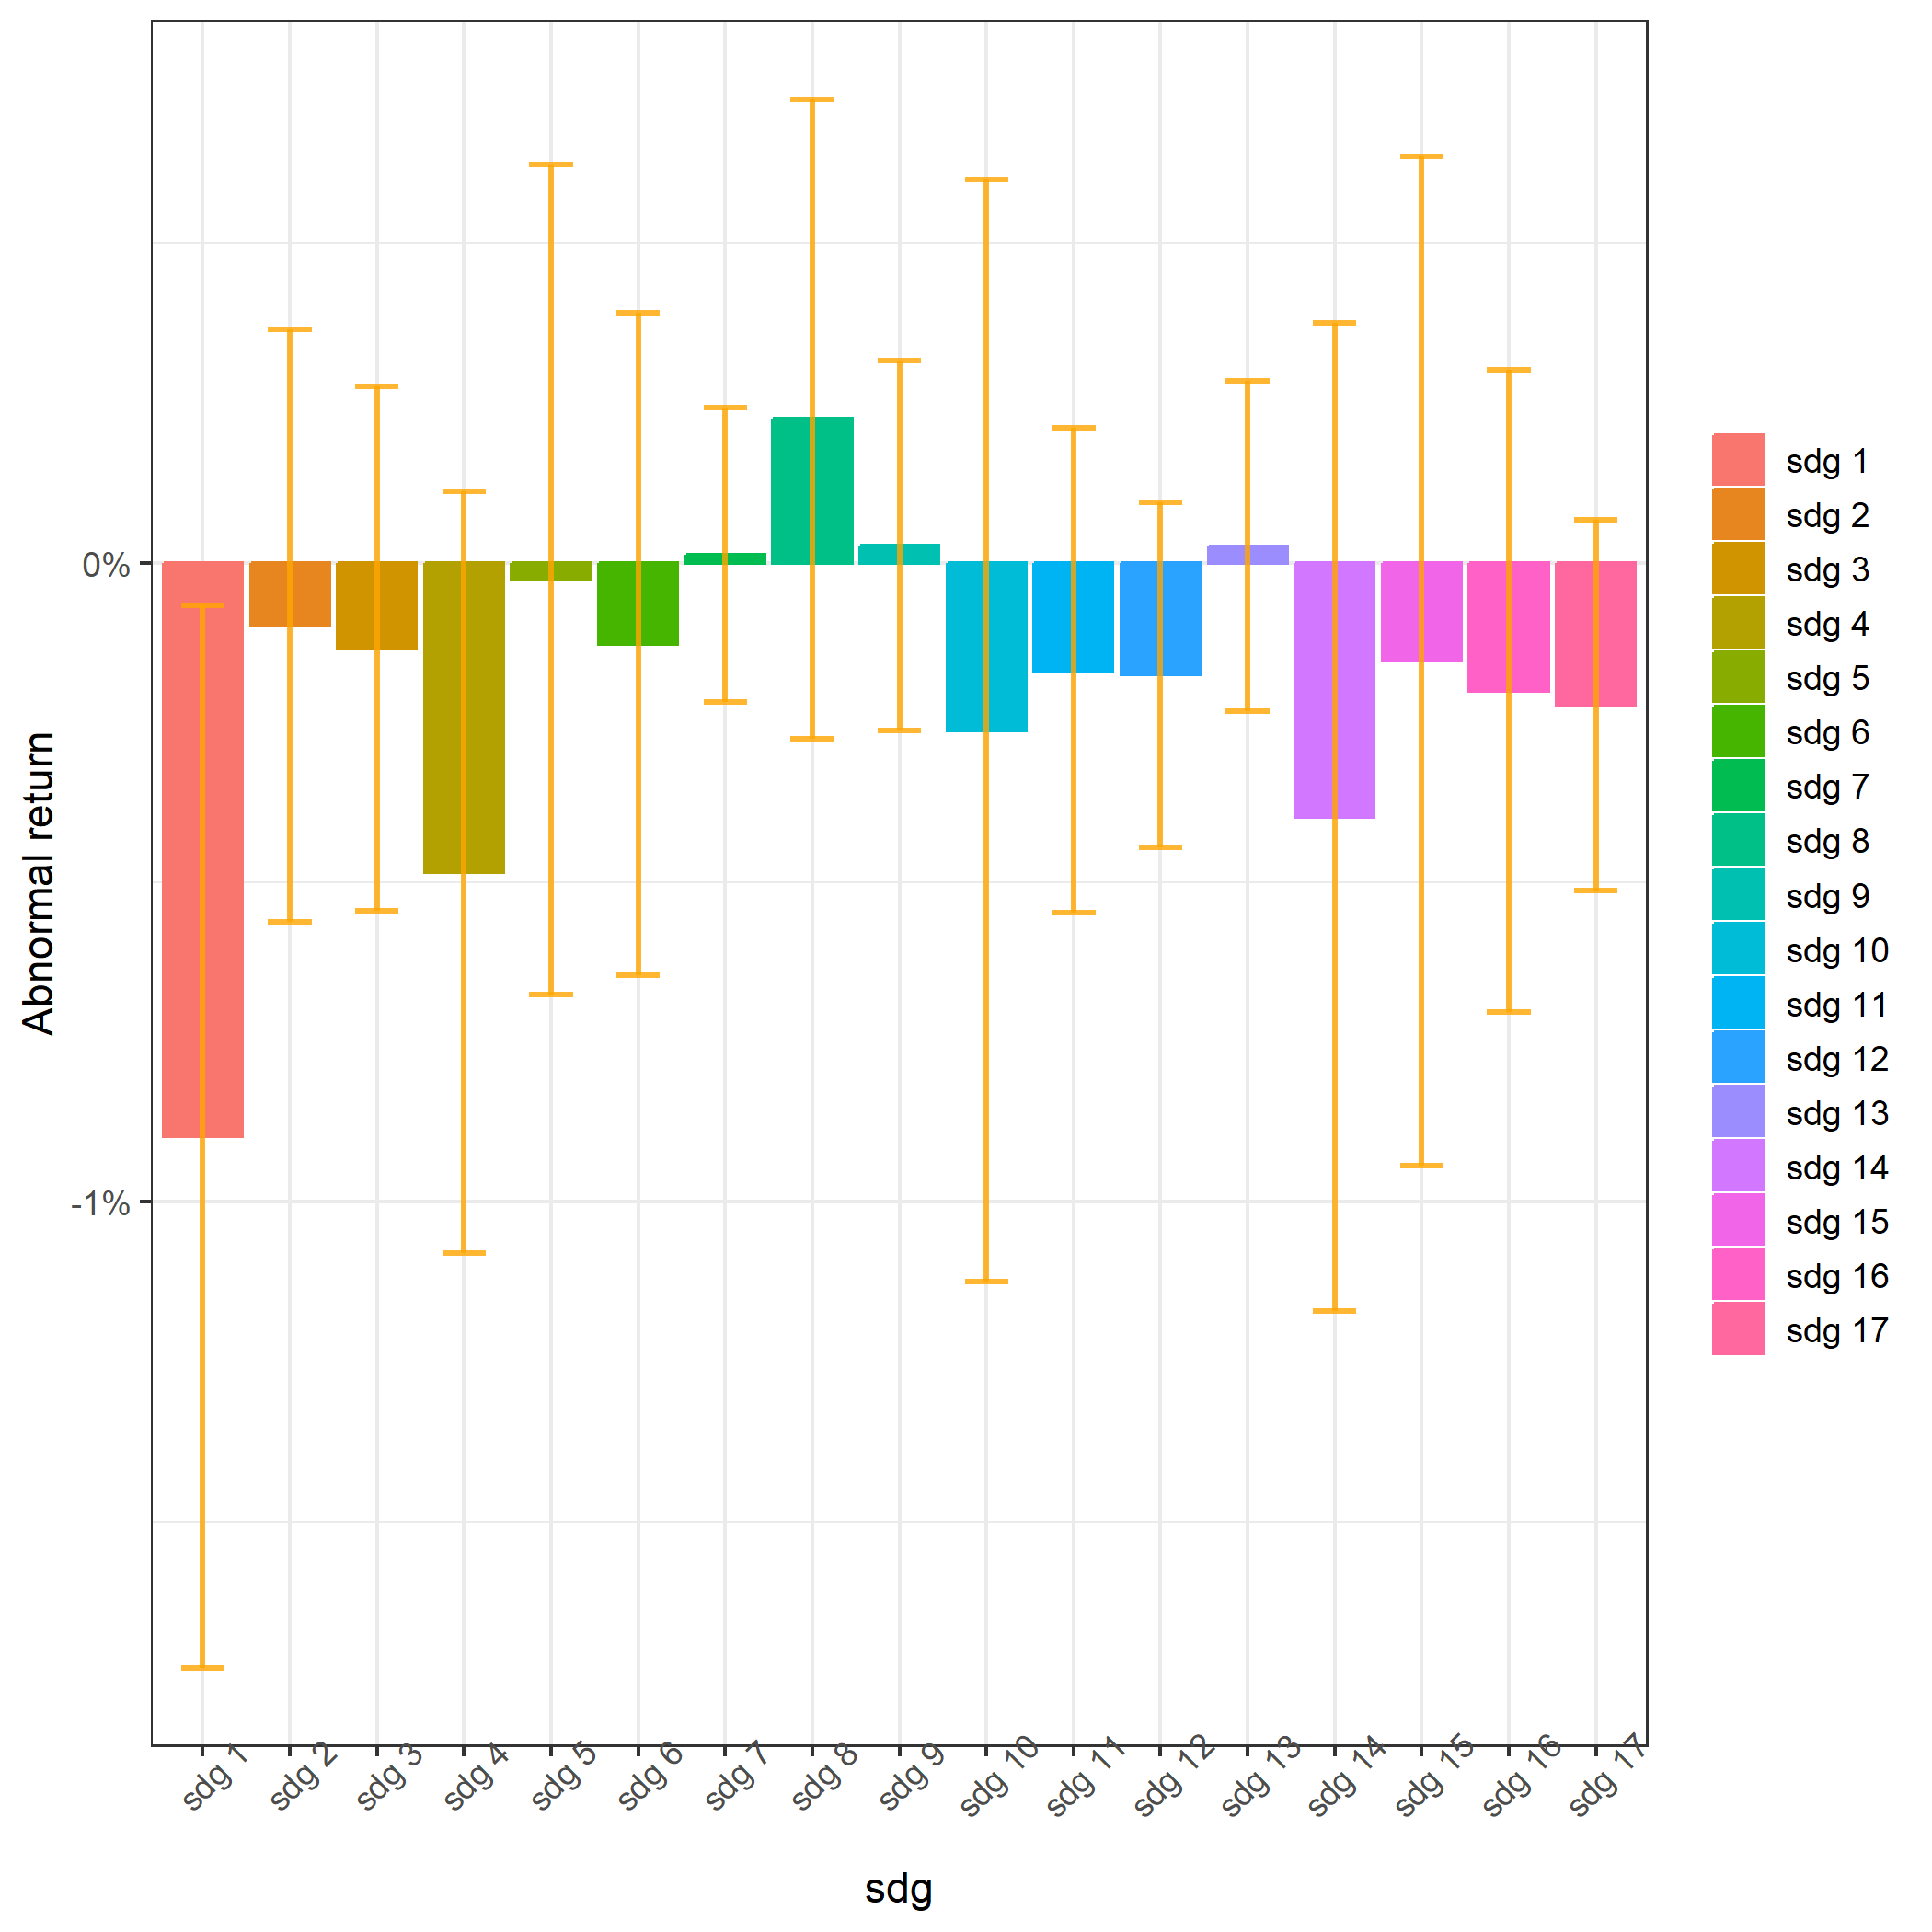
\includegraphics[scale=0.6]{Projekt/1.Figures analysis/ST_positive_sdg_bar.png}
    \caption{$CAAR_{t=10}$: short term positive events}
    \label{fig:ST_pos_news}
\end{figure}




% latex table generated in R 4.2.2 by xtable 1.8-4 package
% Mon Mar 13 12:03:11 2023
\begin{table}[ht]
\centering
\begin{tabular}{lrrrr}
  \hline
   & \multicolumn{2}{c}{Positive news} & \multicolumn{2}{c}{Negative news}  \\
  Time & AAR & CAAR & AAR & CAAR \\
 \hline
-10 & -0.0368 & -0.0368 & -0.0539 & -0.0539 \\ 
  -9 & -0.0465 & -0.0833 & 0.0196 & -0.0343 \\ 
  -8 & 0.0454 & -0.0380 & 0.0267 & -0.0077 \\ 
  -7 & 0.0101 & -0.0278 & -0.0042 & -0.0118 \\ 
  -6 & 0.0368 & 0.0090 & -0.0082 & -0.0200 \\ 
  -5 & -0.0037 & 0.0053 & 0.0052 & -0.0148 \\ 
  -4 & 0.0300 & 0.0352 & -0.0910 & -0.1058 \\ 
  -3 & 0.0085 & 0.0437 & -0.0930 & -0.1988 \\ 
  -2 & -0.0204 & 0.0233 & -0.2364 & -0.4348 \\ 
  -1 & 0.0113 & 0.0345 & -0.2184 & -0.6532 \\ 
  0 & 0.0735 & 0.1080 & -0.3604 & -1.0119 \\ 
  +1 & -0.0296 & 0.0790 & -0.0833 & -1.0952 \\ 
  +2 & -0.0496 & 0.0282 & -0.0232 & -1.1150 \\ 
  +3 & -0.0440 & -0.0147 & 0.1148 & -0.9901 \\ 
  +4 & -0.0174 & -0.0315 & 0.0313 & -0.9588 \\ 
  +5 & -0.0002 & -0.0321 & -0.0087 & -0.9675 \\ 
  +6 & -0.0466 & -0.0793 & 0.0385 & -0.9282 \\ 
  +7 & -0.0492 & -0.1242 & 0.0200 & -0.9083 \\ 
  +8 & 0.0000 & -0.1271 & 0.0261 & -0.8822 \\ 
  +9 & -0.0127 & -0.1368 & -0.0191 & -0.9013 \\ 
  +10 & -0.0241 & -0.1641 & 0.0185 & -0.8885 \\ 
   \hline
\end{tabular}
\caption{AAR and CAAR over event window (in percentage)} 
\end{table}

 \label{ST_tab}

\subsubsection{Negative news}

The effect from negative events is clearly more influential on shareholder sentiment than positive events. Figure \ref{fig:ST_pos_news} illustrates the development in AAR and CAAR.  The impact from negative events is approximately zero until $t = -6$ upon which the AAR decreases steadily until $t=0$, where it bottoms at $-0.36\%$. Subsequently, after the negative event at $t=0$ the AAR increases towards $0.0\%$ and remains there for the rest of the periods. The CAAR stays negative during the full event window and bottoms at $t=2$ after a large decline of approximately $1.2\%$ from  $t=-5$.  
Moreover, the AAR is significantly negative between $t=-2$ and $t=0$ at $95\%$. The same goes for the CAAR after $t=-2$ and the remaining window.  

\begin{figure} [H]
    \centering
    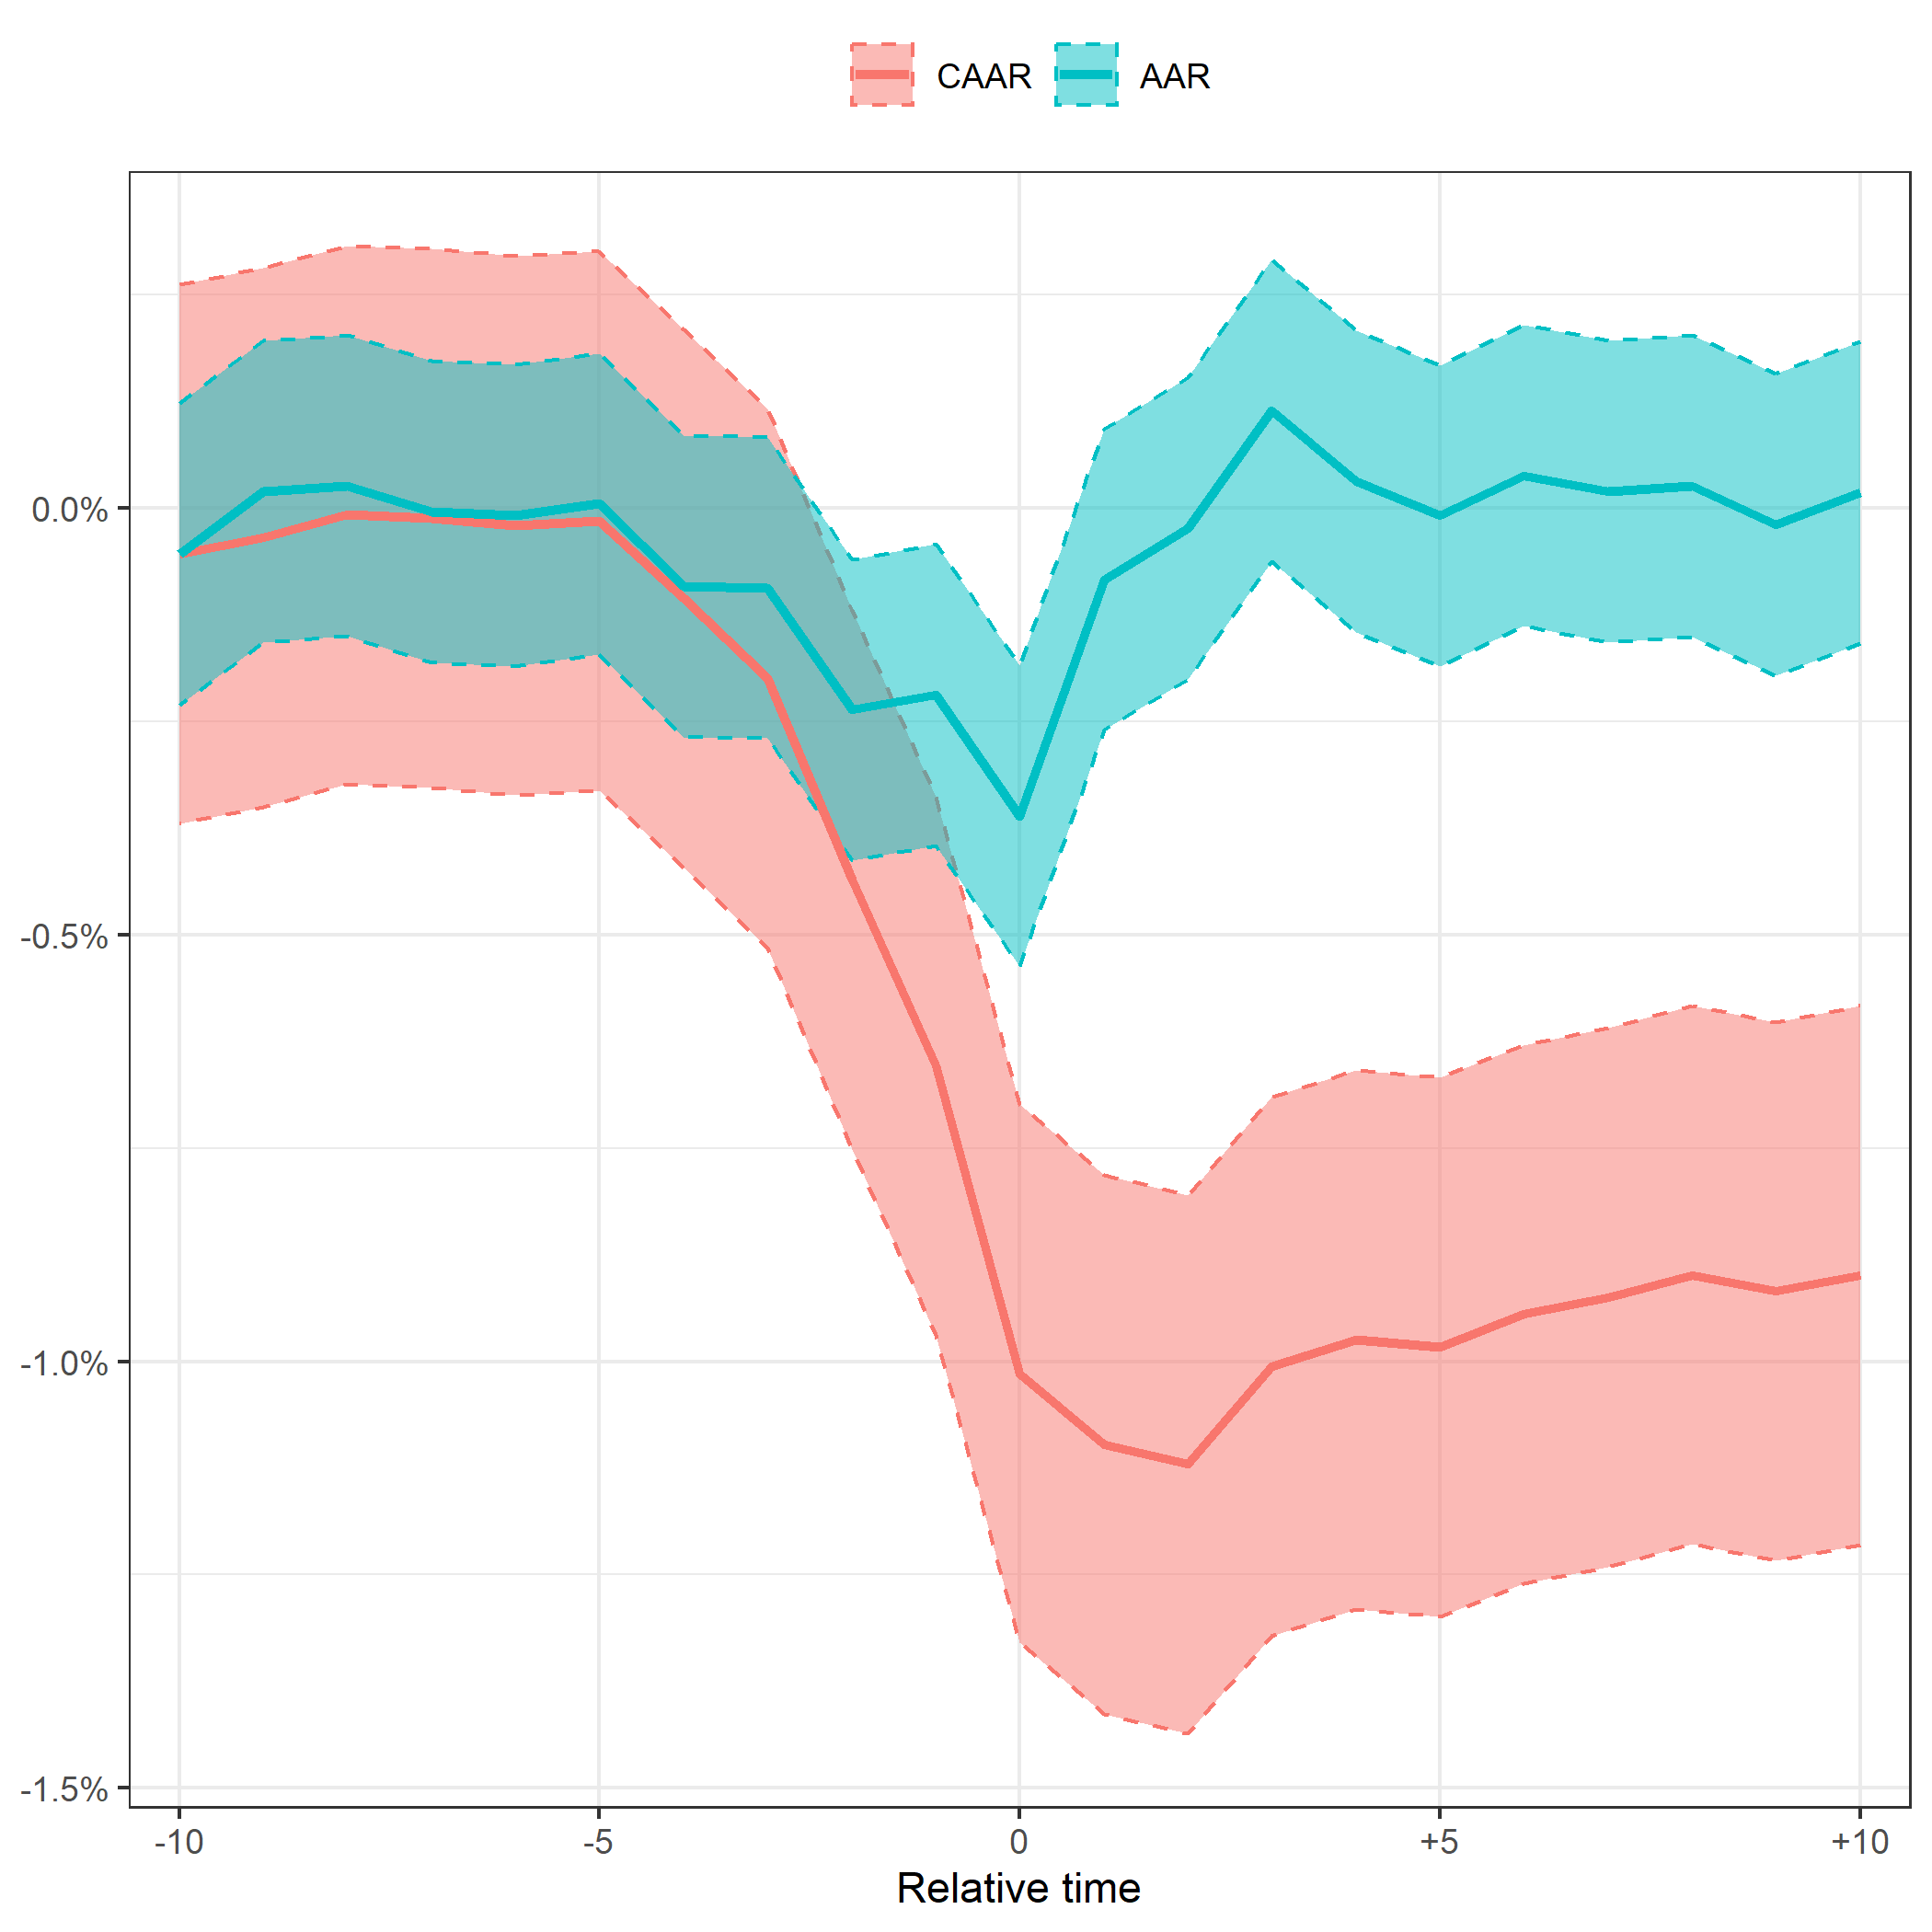
\includegraphics[scale=0.6]{Projekt/1.Figures analysis/ST_negative_all_CI.png}
    \caption{Short term negative news: AAR and CAAR}
    \label{fig:ST_neg_news}
\end{figure}


\subsection{Individual SDGs}

The individual SDGs


\begin{figure} [H]
    \centering
    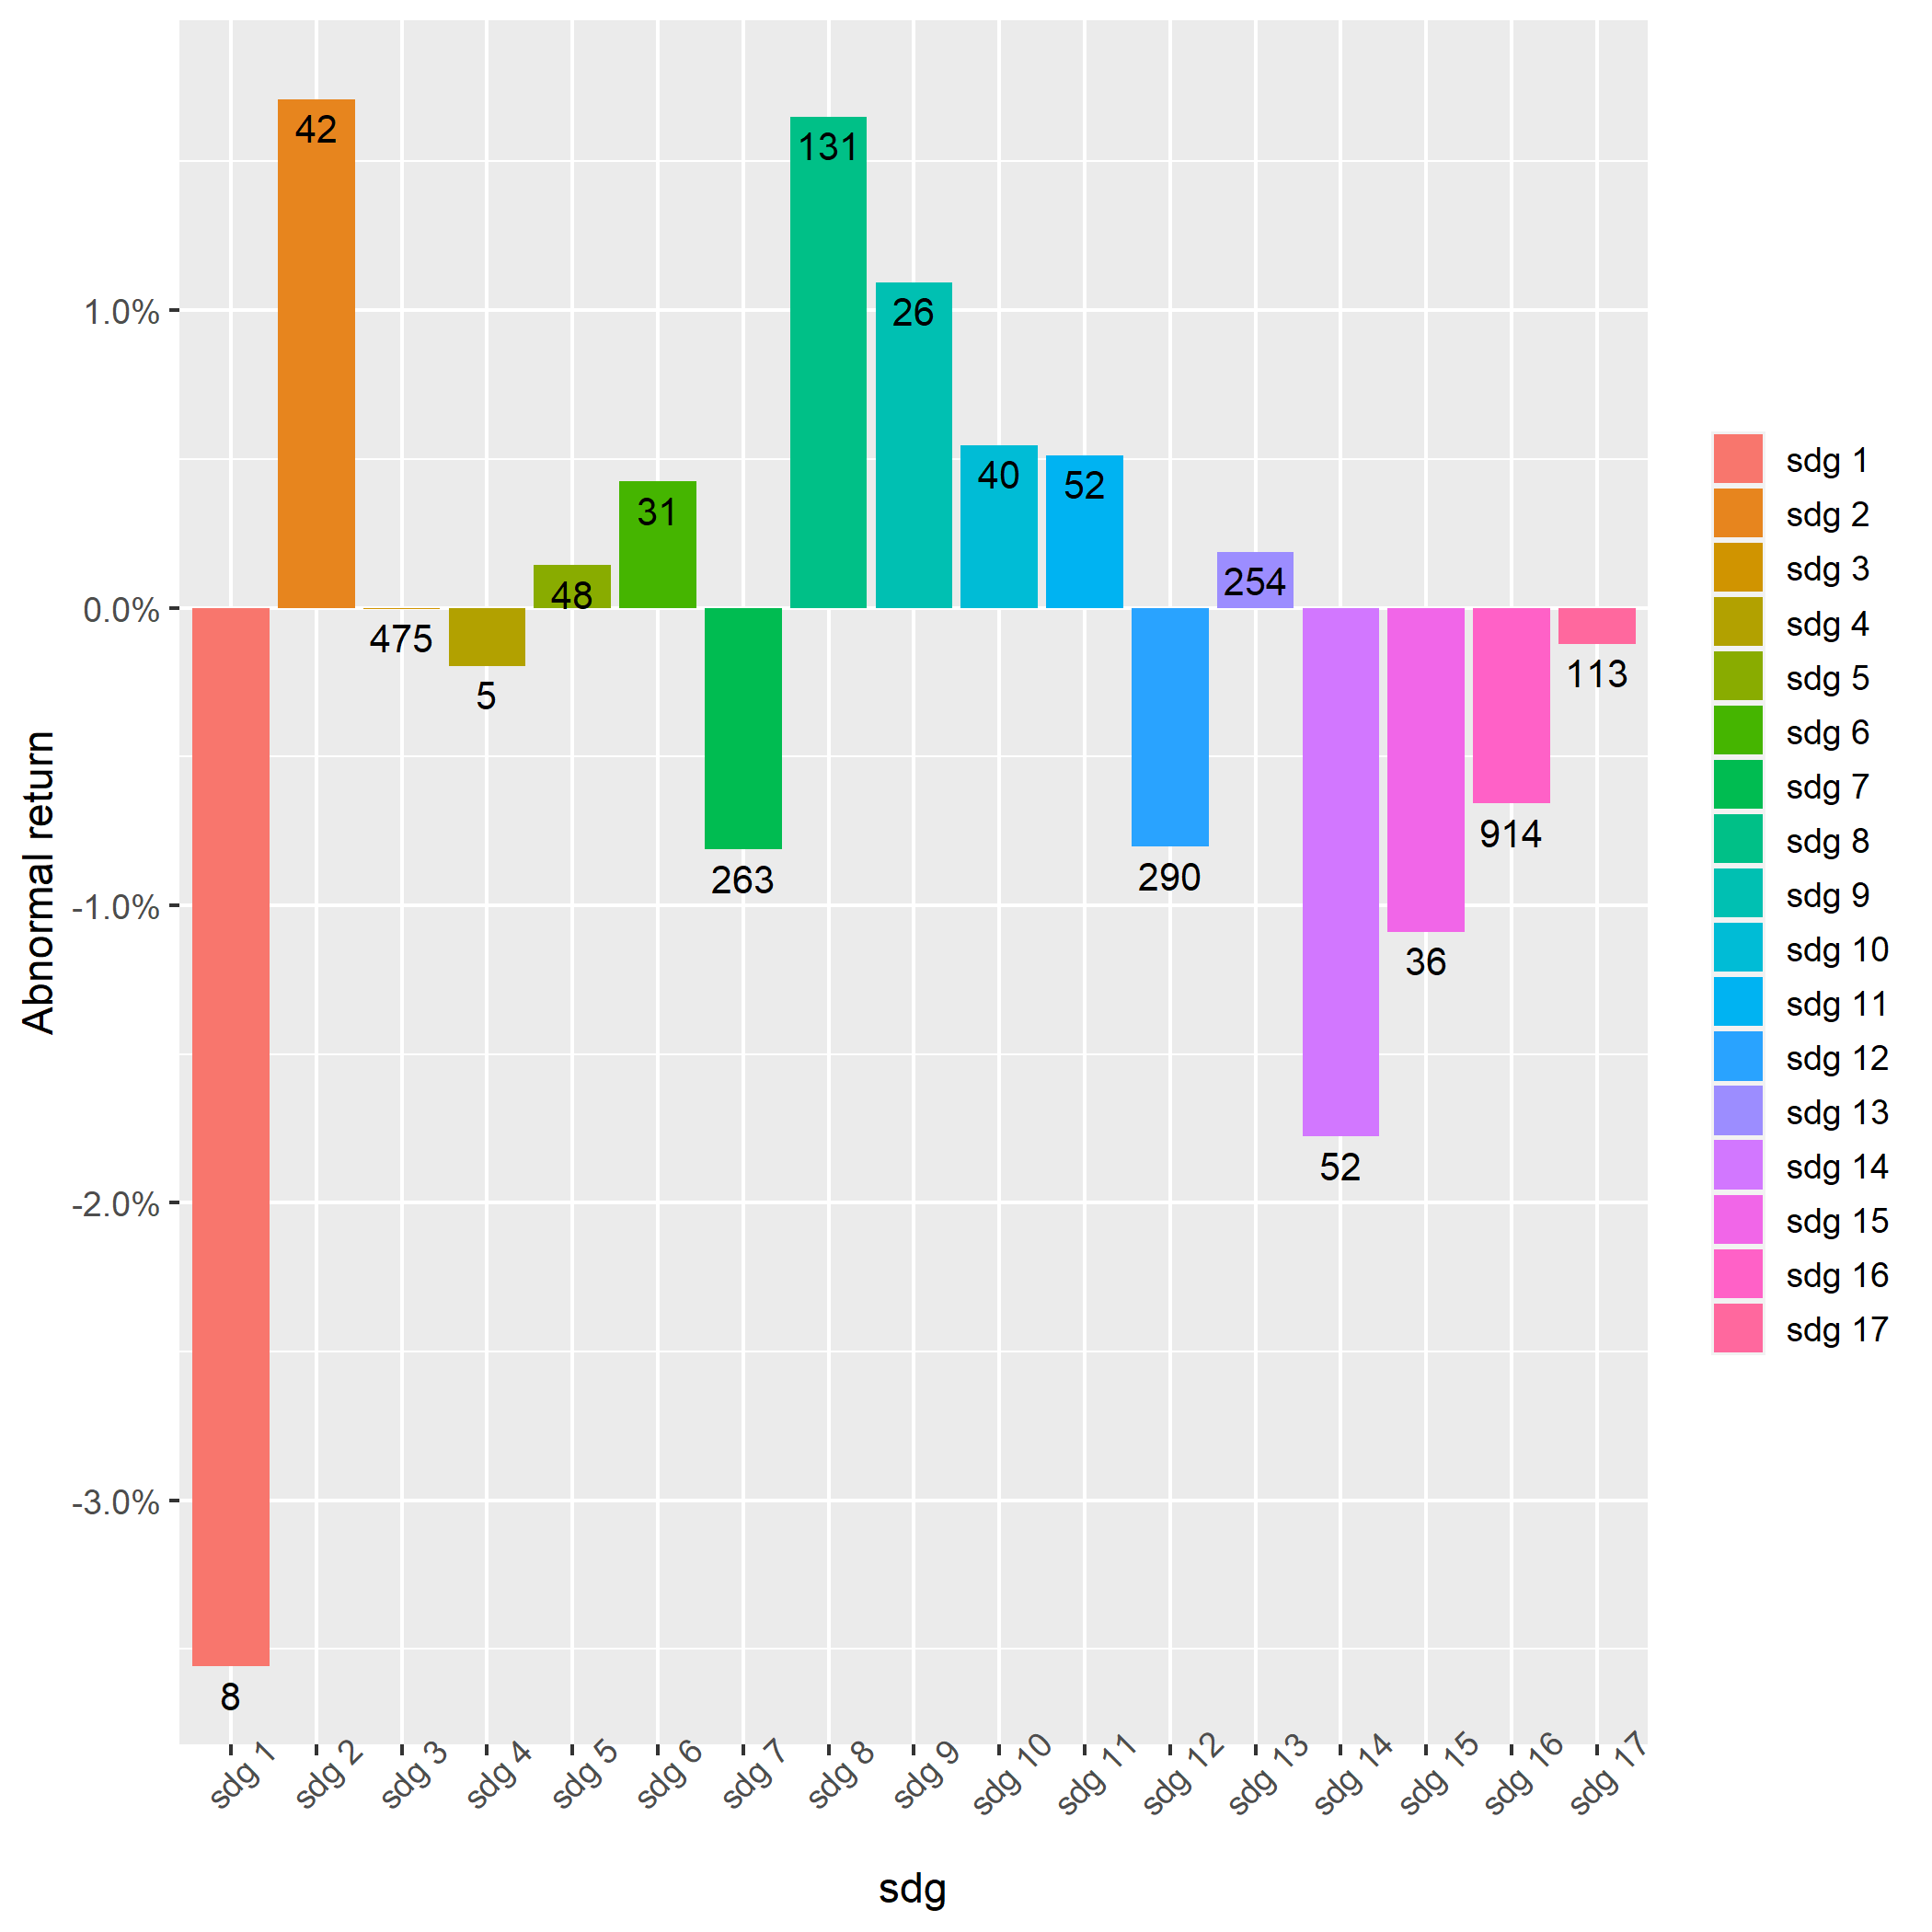
\includegraphics[scale=0.6]{Projekt/1.Figures analysis/ST_negative_sdg_bar.png}
    \caption{CAAR short term negative news}
    \label{fig:ST_pos_news}
\end{figure}




